\documentclass[10pt,hyperref={CJKbookmarks=true},xcolor=dvipsnames,aspectratio=169]{beamer}
\usetheme[navigation]{UMONS}
\usepackage[utf8]{inputenc}
\usepackage{verbatim}
\usepackage{ctex}

\title[国际经济学]{国际经济学}
\subtitle{汇率与外汇市场}
\author{鲁晓东}
\institute[]{%
	岭南学院\hspace{2em}中山大学
	\\[4ex]
	
\includegraphics[height=8ex]{fig/lingnanlogo}\hspace{2em}%
	
\includegraphics[height=8.5ex]{fig/sysu}
}
%------------section前展示一页----------
\AtBeginSection[] {     
	\begin{frame}        
	\tableofcontents[currentsection,hideallsubsections]    
\end{frame} 
}

%-------------subsection也展示一下----------
\AtBeginSubsection[]{

\frame<beamer>{ 
	
	\frametitle{Outline}   
	
	\tableofcontents[currentsection,currentsubsection] 
	
}

}
%---------------------------

%-----------一段一闪现-------
%\beamerdefaultoverlayspecification{<+->}
%这个功能基本不用

\begin{document}
\maketitle


\begin{frame}
\frametitle{提纲}
\tableofcontents
\end{frame}				%生成提纲页

%-----------正文开始----------------------

%\beamerdefaultoverlayspecification{<+->}
\section{Motivation}
\frame{
	\frametitle{Fixed Exchange Rate }
	\begin{figure}
		\centering
		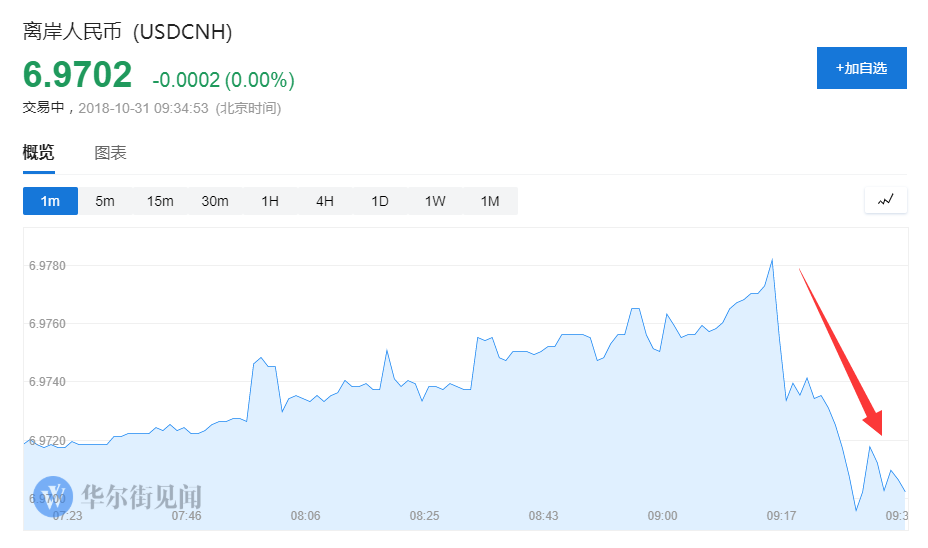
\includegraphics[scale=0.32]{fig/exchange/rmb}
	\end{figure}
}

\begin{frame}{人民币何时破七}
\begin{block}{华尔街见闻10月31日财经资讯}
	
	\textbf{离岸人民币收复6.97关口 中间价续创2008年以来新低}\\
	\small
	10月31日周三早盘,离岸人民币兑美元快速反弹逾90点,收复6.97关口,报6.9695。此前中国央行宣布下周在港发行央票。\\
	在岸人民币兑美元开盘报6.9639;人民币中间价连续第二日下调,两日累计下调269点,报6.9646,为2008年以来最低。上一交易日中间价6.9574;上一交易日官方收盘价报6.9613,上一交易日夜盘收盘报6.9675。
	
	此前一天,受G20峰会相关负面消息、人民币中间价下调影响,在岸人民币一度跌至6.9717,创逾10年来最低。
	
	年初迄今,美元指数节节高升,现已升破97,创下2017年6月来新高。
	
	从今年6月中旬至今,人民币兑美元汇率一直呈现贬值走势,四个月累计贬值超过8\%。
\end{block}
\begin{itemize}
	\item 何为人民币中间价?何为开盘,何为收盘?何为离岸人民币?人民币的标准代码应该是CNY还是CNH?
	\item 人民币中间价从6.9639变为6.9646,明明是变大了,为何称为“下调”
	\item 269点是个什么意思?有必要搞这么精确吗?
	\item 7这个数字是人民币的幸运数字吗?
	\item 最近4个月来,人民币为何持续贬值?如果你是央行主席,是否应该出面干预?如何干预?
\end{itemize}
\end{frame}

\frame{
	\frametitle{Turnover by currencies and currency pairs }
	\begin{figure}
		\centering
		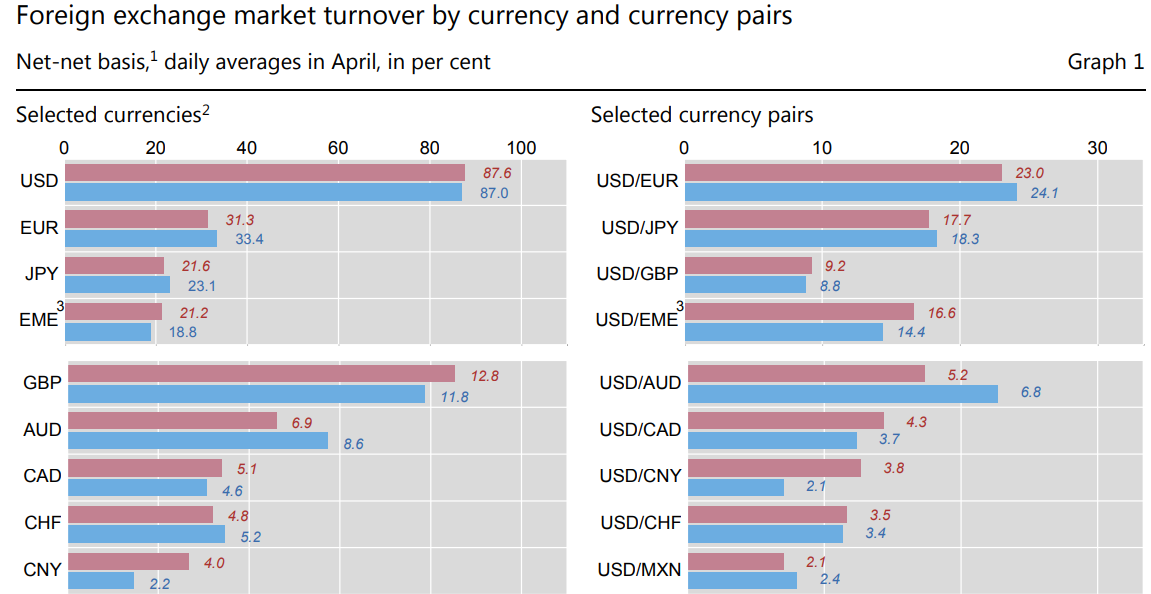
\includegraphics[scale=0.4]{fig/exchange/rank}
	\end{figure}
}

\frame{
	\frametitle{Turnover by instrument and maturity  }
	\begin{figure}
		\centering
		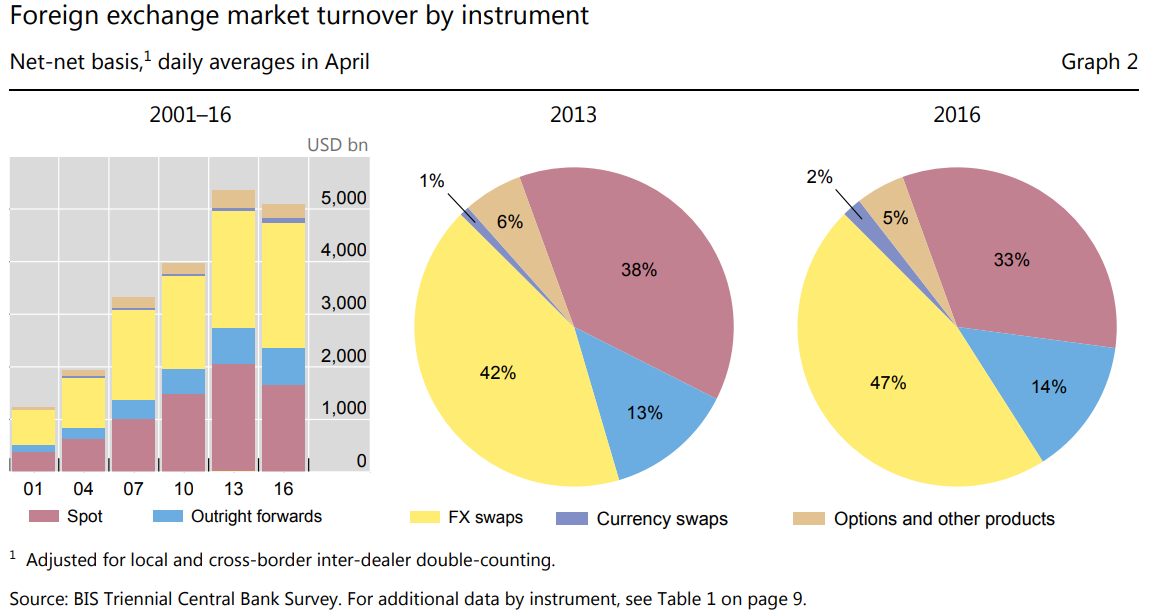
\includegraphics[scale=0.4]{fig/exchange/rank2}
	\end{figure}
}

\frame{
	\frametitle{Turnover by counterparty  }
	\begin{figure}
		\centering
		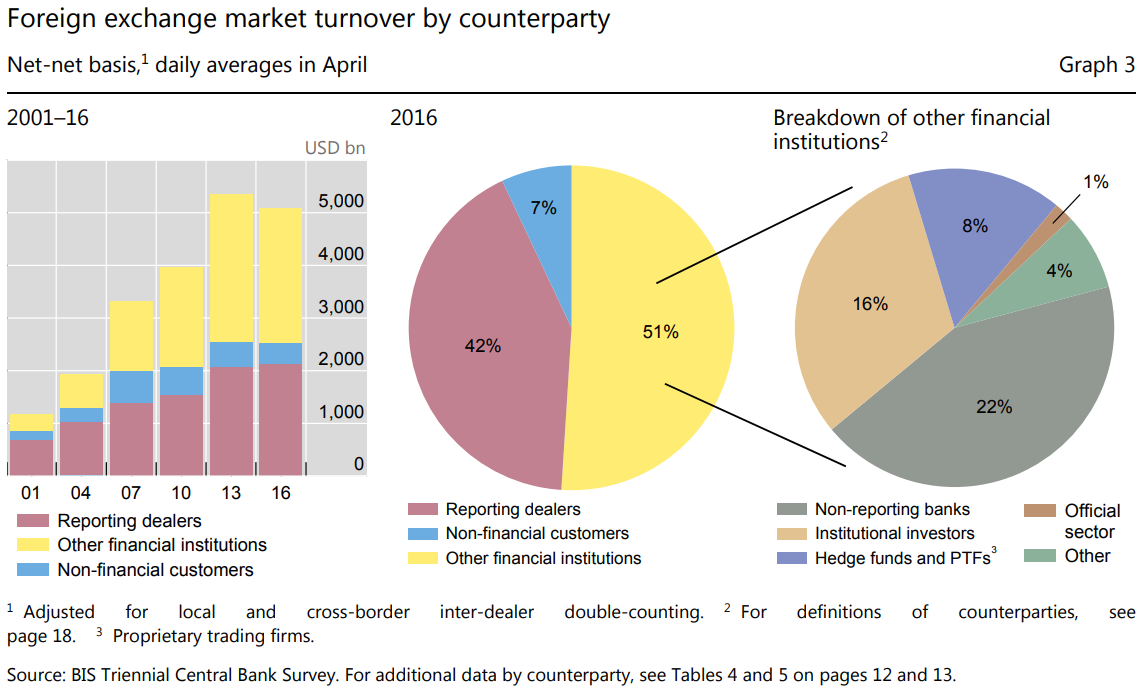
\includegraphics[scale=0.35]{fig/exchange/rank3}
	\end{figure}
}

\frame[plain]{% how to print
	\frametitle{}
	\begin{center}
		\textcolor{blue}{Chapter 14: Exchange Rates and the Foreign Exchange Market: An Asset Approach }
	\end{center}
}


\section{Exchange Rate}

\frame{
	\frametitle{Exchange Rates}
	\begin{itemize}
		\item Defination: \structure{exchange rate} is simply the price of one currency in terms of another, and there
		are two methods of expressing it:
		\begin{enumerate}
					\item \textit{Direct}: The price of the foreign currency in terms
			of CNY (e.g., $6.97$ CNY per USD): $E_{CNY/USD}$
			\item \textit{Indirect} : The price of CNY in terms of the foreign currency (e.g., $0.1434$ US dollar per 1 CNY)
		\end{enumerate}

	\end{itemize}
	Exchange rate regimes:
	\begin{itemize}
		\item \textit{flexible}: Exchange rate is determined freely by the market
		\item \textit{fixed}: Exchange rate is politically determined and market is manipulated
	\end{itemize}
}

\frame{
	\frametitle{the Recent Summary of RMB }
	\begin{figure}
		\centering
		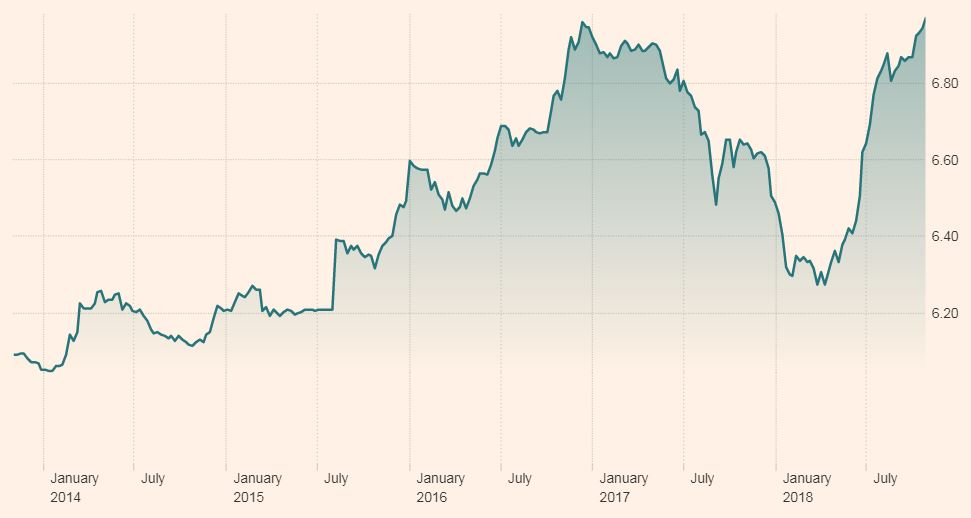
\includegraphics[scale=0.5]{fig/exchange/usrmb.jpg}
	\end{figure}
}

\frame{
	\frametitle{the Long-run Tendency of RMB }
	\begin{figure}
		\centering
		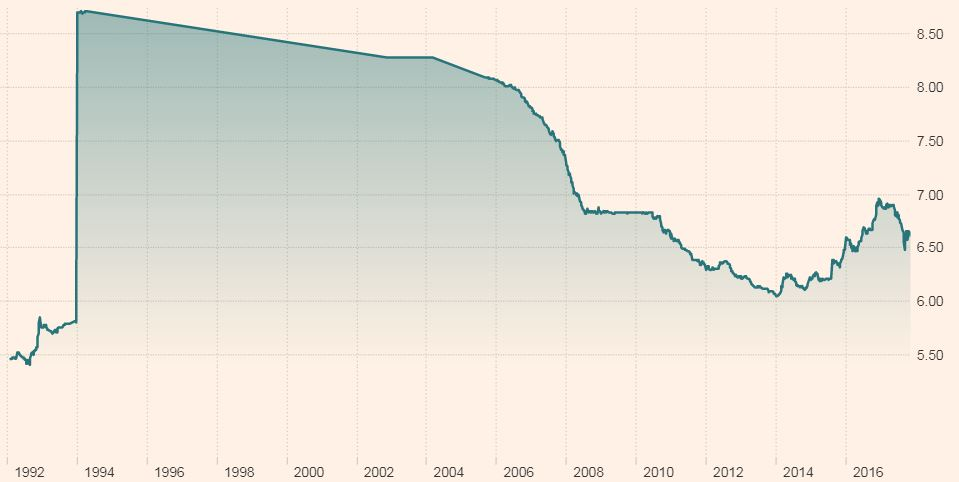
\includegraphics[scale=0.5]{fig/exchange/usrmb2}
	\end{figure}
}

\frame{
	\frametitle{Exchange Rate Quotations}
	\begin{figure}
		\centering
		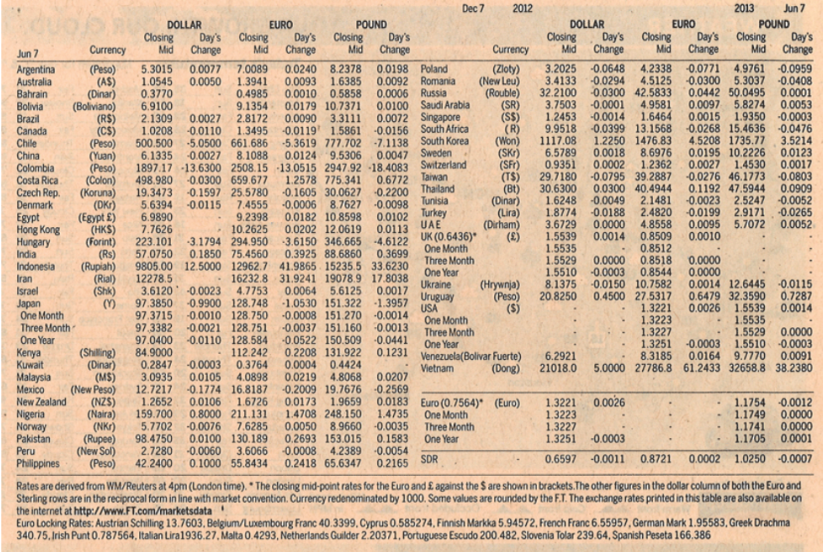
\includegraphics[scale=0.5]{fig/exchange/ft_ex.png}
		\label{fig:11}
	\end{figure}
}

\frame{
	\frametitle{Depreciation and Appreciation}
	If we are under \textbf{flexible exchange rates}:
	\begin{enumerate}
		\item \textbf{Depreciation} $E_{CNY/USD} \Uparrow$ the US dollar becomes more
		expensive, i.e., RMB becomes less valuable.
		\item \textbf{Appreciation} $E_{CNY/USD} \Downarrow$ the US dollar becomes less
		expensive, i.e., RMB becomes more
		valuable.
	\end{enumerate}
}


\frame{
	\frametitle{Devaluation and Revaluation}
	If we are under \textbf{fixed exchange rates}:
	\begin{enumerate}
		\item \textbf{Devaluation} $E_{CNY/USD} \Uparrow$ the Euro becomes more
		expensive, i.e., CNY becomes less valuable.
		\item \textbf{Revaluation} $E_{CNY/USD} \Downarrow$ the Euro becomes less
		expensive, i.e., CNY becomes more		valuable.
	\end{enumerate}
}
\section{Foreign Exchange Market}

\subsection{Parties involved in 外汇市场}

\frame{
	\frametitle{The Foreign Exchange Market}
	Main actor:
	\begin{itemize}
		\item \textbf{Commercial banks and other depository institutions}
		\begin{itemize}
			\item Suppose I want to buy some books from Amazon US
			\item ABC charges me in CNY, and then pays Amazon in USD
		\end{itemize}
		\item Interbank trading is lions share of foreign currency trading
		\item \emph{Wholesale} rates in the Financial Times: only trades of high amount
		\item \emph{Retail} rates available to you and I are much worse
\end{itemize}}

\frame{
	\frametitle{The Foreign Exchange Market}
	Other actors:
	\begin{enumerate}
		\item \textbf{Non-financial businesses} directly buy foreign currency transactions to pay foreign employees or suppliers 
		\item \textbf{Non-bank financial institutions} may trade foreign currency for investment clients
		\item \textbf{Central banks} conduct official international reserves trades (small)
	\end{enumerate}
}

\frame{
	\frametitle{Characteristics of the Foreign Exchange Market}
	\begin{itemize}
		\item Incredible volume
		\begin{itemize}
			\item 4 trillion USD traded a day
			\item The value of everything produced in the world in a year -- 70 trillion dollars
		\end{itemize}
		\item Tightly connected market
		\begin{itemize}
			\item Price cannot be different in different places
			\item No \emph{arbitrage}
			\item That is, can't buy in London, sell in Copenhagen for a profit
		\end{itemize}
	\end{itemize}
}
\begin{frame}{THE FOREIGN EXCHANGE MARKET}

\begin{itemize}
	\item One of the most fascinating things about the foreign exchange market
	is the huge sums of money that are exchanged on a daily basis. 
	\begin{figure}
		
		
		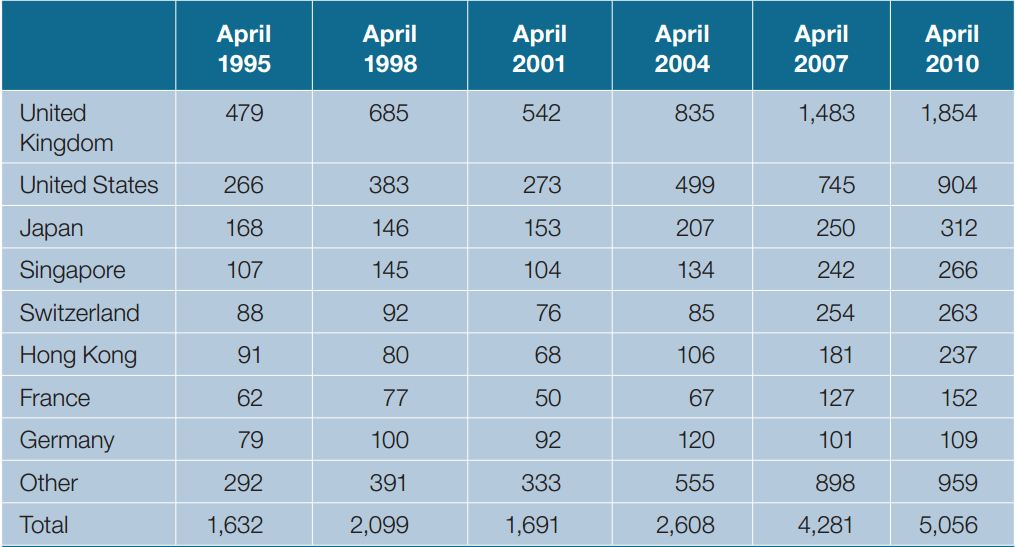
\includegraphics[scale=0.4]{fig/exchange/lec08-1.JPG}
		
	\end{figure}
	
\end{itemize}
\end{frame}

\begin{frame}[plain]{Geographic composition of Foreign exchange market turnover}


\begin{figure}
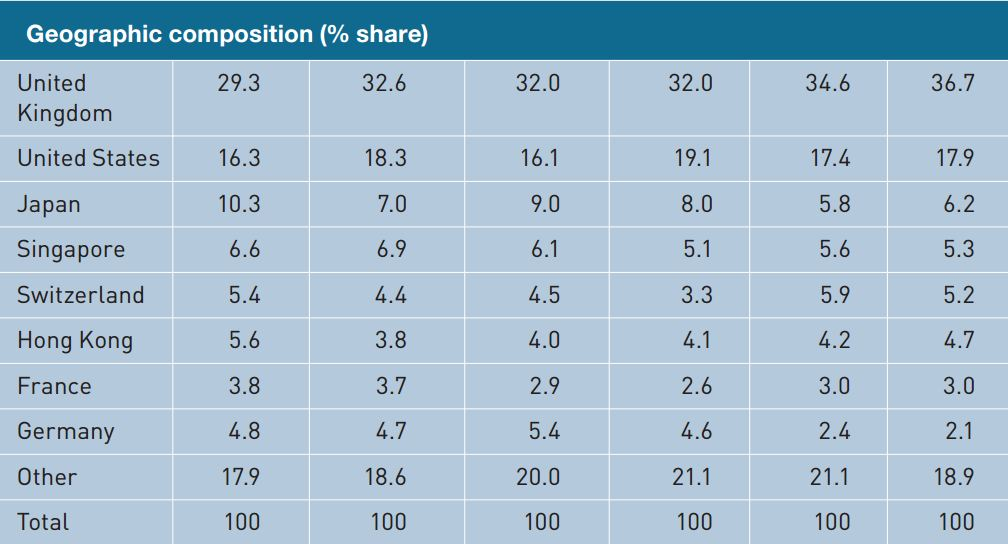
\includegraphics[scale=0.3]{fig/exchange/lec08-2.JPG}
\end{figure}

\begin{itemize}
\item The main centre for foreign exchange trading is London, with some
\$1,854 billion worth of foreign exchange traded on a daily basis,
quite a lot when one considers that the annual gross domestic product
of the United Kingdom only around 50\% more than that.
\item Other important foreign exchange centres are New York with \$904 billion,
Tokyo with \$312 billion, Singapore \$266 billion, Paris \$152 billion
and Frankfurt \$109 billion.
\end{itemize}
\end{frame}

\subsection{Transaction in 外汇市场}
\frame{
	\frametitle{Ways to trading currency}
	\begin{itemize}
		\item \textbf{Spot rate}: exchange rates for currency exchange "on the spot", or when trading is executed immediately.
		\item \textbf{Forward rate}: promise to buy or sell in the future. most commonly for one month (30 days), three months (90 days),
		six months (180 days), nine months (270 days) and one year (360 days). 
		
	\end{itemize}
	Other methods:
	\begin{enumerate}
		\item \textbf{Foreign exchange swap} sell currency on the spot and promise to buy it back in the future
		\item \textbf{Futures contract} Promise to deliver currency in the future
		\item \textbf{Options contracts} Option to buy or sell currency for a fixed rate in the future
	\end{enumerate}
}



\frame{
	\frametitle{Fig. 14-1: Dollar/Pound Spot and 90 Day Forward Exchange Rates, 1983-2013 }
	\begin{itemize}
		\item Why are they so close? It would be explained in CIP theory
	\end{itemize}
	\begin{figure}
		\centering
		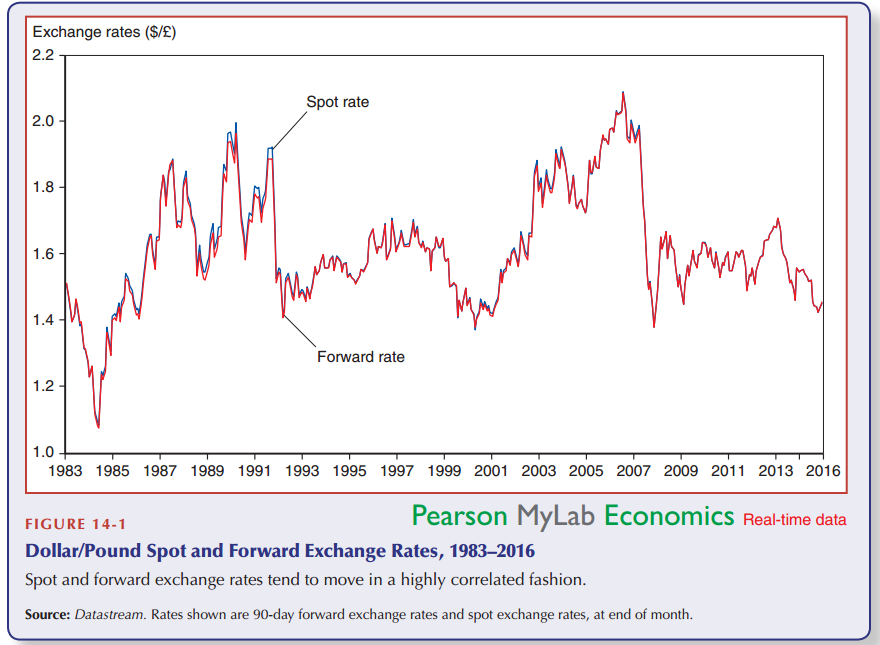
\includegraphics[scale=0.35]{fig/exchange/spot_forward.png}
	\end{figure}
}



\begin{frame}[allowframebreaks]{Other Types Exchange Rate}

\begin{itemize}
	
	\item Nominal exchange rate
	
	\begin{itemize}
		\item The exchange rate that prevails at a given date is known as the nominal
		exchange rate
	\end{itemize}
	\item Real exchange rate
	
	\begin{itemize}
		\item The real exchange rate is the nominal exchange rate adjusted for relative
		prices between the countries under consideration.
		\item It is normally expressed in index form algebraically as:
		\[
		S_{r}=S\frac{P}{P^{*}}
		\]
		
		\item where $S_{r}$ is the index of the real exchange rate, $S$ is the
		nominal exchange rate \textit{\textcolor{magenta}{(foreign currency
				units per unit of domestic currency}}) in index form, $P$ is the
		index of the domestic price level and $P^{*}$ is the index of the
		foreign price level.
	\end{itemize}
	\item Effective exchange rate
	
	\begin{itemize}
		\item a measure of whether or not the currency is appreciating or depreciating
		against \textbf{\textcolor{blue}{a weighted basket}} of foreign currencies. 
	\end{itemize}
	\item Real effective exchange rate index
	
	\begin{itemize}
		\item While the nominal effective exchange rate is easy to compile on a
		daily basis and normally provides a reasonable measure of changes
		in a country’s competitive position for periods of several months
		\item it does not take account of the effect of price movements. 
	\end{itemize}
	

\end{itemize}
\end{frame}





\begin{frame}{Takeaways}
\begin{itemize}
	\item We have seen who trades currency 
	\item We have seen how currency is traded
	\item Then we care about how exchange rate is set?
\end{itemize}
\end{frame}

\end{document}